\documentclass[14pt,fleqn]{extarticle}
\RequirePackage{prepwell-eng}

\previewoff 

\begin{document} 
\begin{snippet}
    \correct
    
    \[ \prob{A} = \prob{A\cap B} + \prob{A\cap B'} \]
    
    \reason
    
    An event $A$ can happen when another event $B$ also happens (see below) 
    \begin{center}
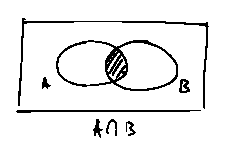
\includegraphics[scale=1.4]{97-A.eps}
\end{center}

Or, $A$ can happen despite $B$ (see below) 
\begin{center}
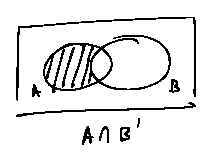
\includegraphics[scale=1.4]{97-B.eps}
\end{center}

There is no third possibility. Which is why 
\[ \qquad \prob{A} = \prob{A\cap B} + \prob{A\cap B'} \]
\end{snippet} 
\end{document} 
